% Options for packages loaded elsewhere
\PassOptionsToPackage{unicode}{hyperref}
\PassOptionsToPackage{hyphens}{url}
%
\documentclass[
]{article}
\usepackage{amsmath,amssymb}
\usepackage{lmodern}
\usepackage{ifxetex,ifluatex}
\ifnum 0\ifxetex 1\fi\ifluatex 1\fi=0 % if pdftex
  \usepackage[T1]{fontenc}
  \usepackage[utf8]{inputenc}
  \usepackage{textcomp} % provide euro and other symbols
\else % if luatex or xetex
  \usepackage{unicode-math}
  \defaultfontfeatures{Scale=MatchLowercase}
  \defaultfontfeatures[\rmfamily]{Ligatures=TeX,Scale=1}
\fi
% Use upquote if available, for straight quotes in verbatim environments
\IfFileExists{upquote.sty}{\usepackage{upquote}}{}
\IfFileExists{microtype.sty}{% use microtype if available
  \usepackage[]{microtype}
  \UseMicrotypeSet[protrusion]{basicmath} % disable protrusion for tt fonts
}{}
\makeatletter
\@ifundefined{KOMAClassName}{% if non-KOMA class
  \IfFileExists{parskip.sty}{%
    \usepackage{parskip}
  }{% else
    \setlength{\parindent}{0pt}
    \setlength{\parskip}{6pt plus 2pt minus 1pt}}
}{% if KOMA class
  \KOMAoptions{parskip=half}}
\makeatother
\usepackage{xcolor}
\IfFileExists{xurl.sty}{\usepackage{xurl}}{} % add URL line breaks if available
\IfFileExists{bookmark.sty}{\usepackage{bookmark}}{\usepackage{hyperref}}
\hypersetup{
  pdftitle={README},
  pdfauthor={LGD},
  hidelinks,
  pdfcreator={LaTeX via pandoc}}
\urlstyle{same} % disable monospaced font for URLs
\usepackage[margin=1in]{geometry}
\usepackage{color}
\usepackage{fancyvrb}
\newcommand{\VerbBar}{|}
\newcommand{\VERB}{\Verb[commandchars=\\\{\}]}
\DefineVerbatimEnvironment{Highlighting}{Verbatim}{commandchars=\\\{\}}
% Add ',fontsize=\small' for more characters per line
\usepackage{framed}
\definecolor{shadecolor}{RGB}{248,248,248}
\newenvironment{Shaded}{\begin{snugshade}}{\end{snugshade}}
\newcommand{\AlertTok}[1]{\textcolor[rgb]{0.94,0.16,0.16}{#1}}
\newcommand{\AnnotationTok}[1]{\textcolor[rgb]{0.56,0.35,0.01}{\textbf{\textit{#1}}}}
\newcommand{\AttributeTok}[1]{\textcolor[rgb]{0.77,0.63,0.00}{#1}}
\newcommand{\BaseNTok}[1]{\textcolor[rgb]{0.00,0.00,0.81}{#1}}
\newcommand{\BuiltInTok}[1]{#1}
\newcommand{\CharTok}[1]{\textcolor[rgb]{0.31,0.60,0.02}{#1}}
\newcommand{\CommentTok}[1]{\textcolor[rgb]{0.56,0.35,0.01}{\textit{#1}}}
\newcommand{\CommentVarTok}[1]{\textcolor[rgb]{0.56,0.35,0.01}{\textbf{\textit{#1}}}}
\newcommand{\ConstantTok}[1]{\textcolor[rgb]{0.00,0.00,0.00}{#1}}
\newcommand{\ControlFlowTok}[1]{\textcolor[rgb]{0.13,0.29,0.53}{\textbf{#1}}}
\newcommand{\DataTypeTok}[1]{\textcolor[rgb]{0.13,0.29,0.53}{#1}}
\newcommand{\DecValTok}[1]{\textcolor[rgb]{0.00,0.00,0.81}{#1}}
\newcommand{\DocumentationTok}[1]{\textcolor[rgb]{0.56,0.35,0.01}{\textbf{\textit{#1}}}}
\newcommand{\ErrorTok}[1]{\textcolor[rgb]{0.64,0.00,0.00}{\textbf{#1}}}
\newcommand{\ExtensionTok}[1]{#1}
\newcommand{\FloatTok}[1]{\textcolor[rgb]{0.00,0.00,0.81}{#1}}
\newcommand{\FunctionTok}[1]{\textcolor[rgb]{0.00,0.00,0.00}{#1}}
\newcommand{\ImportTok}[1]{#1}
\newcommand{\InformationTok}[1]{\textcolor[rgb]{0.56,0.35,0.01}{\textbf{\textit{#1}}}}
\newcommand{\KeywordTok}[1]{\textcolor[rgb]{0.13,0.29,0.53}{\textbf{#1}}}
\newcommand{\NormalTok}[1]{#1}
\newcommand{\OperatorTok}[1]{\textcolor[rgb]{0.81,0.36,0.00}{\textbf{#1}}}
\newcommand{\OtherTok}[1]{\textcolor[rgb]{0.56,0.35,0.01}{#1}}
\newcommand{\PreprocessorTok}[1]{\textcolor[rgb]{0.56,0.35,0.01}{\textit{#1}}}
\newcommand{\RegionMarkerTok}[1]{#1}
\newcommand{\SpecialCharTok}[1]{\textcolor[rgb]{0.00,0.00,0.00}{#1}}
\newcommand{\SpecialStringTok}[1]{\textcolor[rgb]{0.31,0.60,0.02}{#1}}
\newcommand{\StringTok}[1]{\textcolor[rgb]{0.31,0.60,0.02}{#1}}
\newcommand{\VariableTok}[1]{\textcolor[rgb]{0.00,0.00,0.00}{#1}}
\newcommand{\VerbatimStringTok}[1]{\textcolor[rgb]{0.31,0.60,0.02}{#1}}
\newcommand{\WarningTok}[1]{\textcolor[rgb]{0.56,0.35,0.01}{\textbf{\textit{#1}}}}
\usepackage{graphicx}
\makeatletter
\def\maxwidth{\ifdim\Gin@nat@width>\linewidth\linewidth\else\Gin@nat@width\fi}
\def\maxheight{\ifdim\Gin@nat@height>\textheight\textheight\else\Gin@nat@height\fi}
\makeatother
% Scale images if necessary, so that they will not overflow the page
% margins by default, and it is still possible to overwrite the defaults
% using explicit options in \includegraphics[width, height, ...]{}
\setkeys{Gin}{width=\maxwidth,height=\maxheight,keepaspectratio}
% Set default figure placement to htbp
\makeatletter
\def\fps@figure{htbp}
\makeatother
\setlength{\emergencystretch}{3em} % prevent overfull lines
\providecommand{\tightlist}{%
  \setlength{\itemsep}{0pt}\setlength{\parskip}{0pt}}
\setcounter{secnumdepth}{-\maxdimen} % remove section numbering
\ifluatex
  \usepackage{selnolig}  % disable illegal ligatures
\fi

\title{README}
\author{LGD}
\date{17/12/2021}

\begin{document}
\maketitle

{
\setcounter{tocdepth}{3}
\tableofcontents
}
\href{https://www.repostatus.org/\#active}{\includegraphics{https://www.repostatus.org/badges/latest/active.svg}}

\href{https://codecov.io/gh/somaSystems/lifeTimes}{\includegraphics{https://codecov.io/gh/somaSystems/lifeTimes/branch/main/graph/badge.svg?token=4LFWpvvLOq}}


\includegraphics[width=0.4\textwidth,height=\textheight]{man/figures/lifeTimesLogo.png}

This is a package for \textbf{detecting} and \textbf{visualising}
correlations between objects in biological series data.

\textbf{Citation}

\textbf{lifeTimes} is available for everyone. If you find it useful for
your research please cite the work that motivated its development:
\textbf{Environmentally dependent and independent control of cell shape
determination by Rho GTPase regulators in melanoma.} doi:
\url{https://doi.org/10.1101/2021.10.11.463377}

\hypertarget{quick-start}{%
\subsection{\texorpdfstring{\textbf{Quick
start}}{Quick start}}\label{quick-start}}

\protect\hyperlink{}{Back to top}

\textbf{Install lifeTimes}

\begin{Shaded}
\begin{Highlighting}[]
\CommentTok{\#install devtools if needed}
\ControlFlowTok{if}\NormalTok{(}\SpecialCharTok{!}\FunctionTok{require}\NormalTok{(}\StringTok{"devtools"}\NormalTok{)) }\FunctionTok{install.packages}\NormalTok{(}\StringTok{"devtools"}\NormalTok{)}

\CommentTok{\#load devtools}
\FunctionTok{library}\NormalTok{(devtools)}

\CommentTok{\#install dependency from github}
\FunctionTok{install\_github}\NormalTok{(}\StringTok{"jokergoo/ComplexHeatmap"}\NormalTok{)}

\CommentTok{\#install lifeTimes from github, using package access token}
\FunctionTok{install\_github}\NormalTok{(}\StringTok{"somaSystems/lifeTimes"}\NormalTok{, }
\AttributeTok{auth\_token =} \StringTok{"\textless{}paste your github token as a string here\textgreater{}"}\NormalTok{) }

\CommentTok{\# If you need a github token you make one with the commented code below:}
\CommentTok{\# usethis::create\_github\_token() }
\end{Highlighting}
\end{Shaded}

\textbf{Run lifeTimes on default data}

\begin{Shaded}
\begin{Highlighting}[]
\CommentTok{\#copy and paste to run on test data}
\FunctionTok{library}\NormalTok{(lifeTimes)}

\NormalTok{lts }\OtherTok{\textless{}{-}} \FunctionTok{lts\_in}\NormalTok{() }\CommentTok{\#calculate cross correlation}
\end{Highlighting}
\end{Shaded}

\textbf{Visualise results from lifeTimes on default data}

\begin{Shaded}
\begin{Highlighting}[]
\FunctionTok{lts\_plot\_ccfs}\NormalTok{(lts) }\CommentTok{\#plot clustered correlations}
\end{Highlighting}
\end{Shaded}

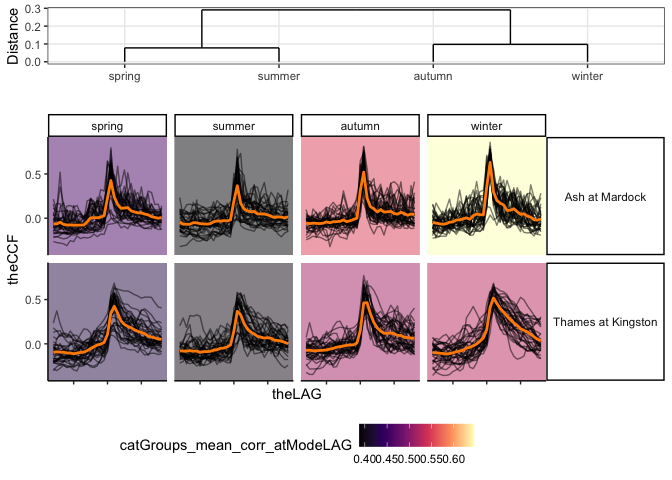
\includegraphics{htmlREADME_files/figure-latex/unnamed-chunk-3-1.pdf}

\begin{Shaded}
\begin{Highlighting}[]
\FunctionTok{lts\_plot\_ClustSum}\NormalTok{(lts) }\CommentTok{\#plot direction of correlations}
\end{Highlighting}
\end{Shaded}

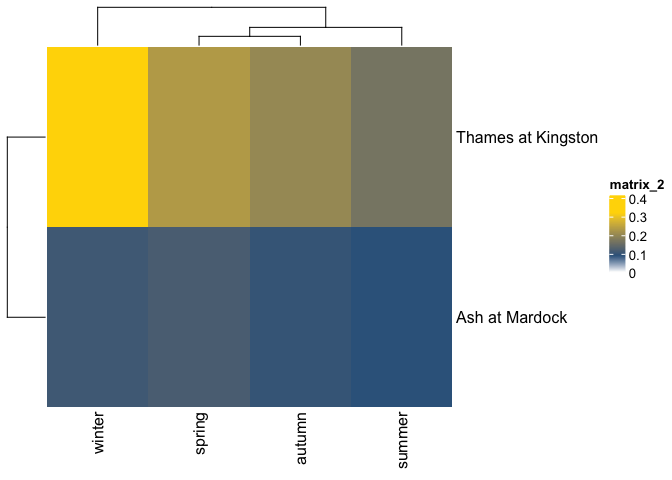
\includegraphics{htmlREADME_files/figure-latex/unnamed-chunk-3-2.pdf}

\begin{Shaded}
\begin{Highlighting}[]
\FunctionTok{lts\_plot\_coupled}\NormalTok{(lts) }\CommentTok{\# plot strength and direction of correlation}
\end{Highlighting}
\end{Shaded}

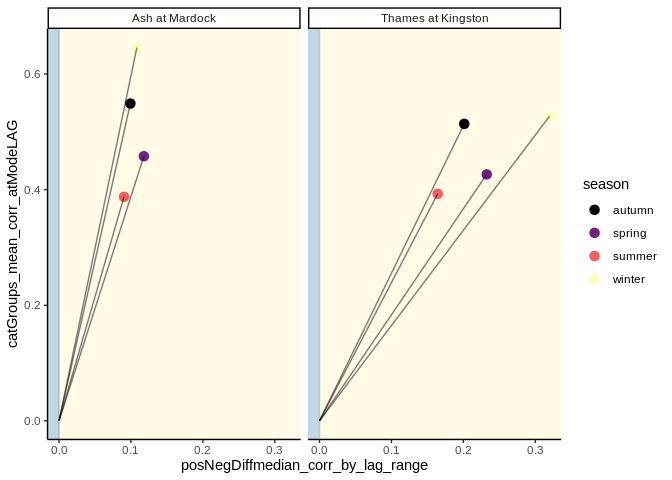
\includegraphics{htmlREADME_files/figure-latex/unnamed-chunk-3-3.pdf}

\textbf{Fig 1} Ariel images of the Ash, and Thames rivers.

\begin{figure}
\centering
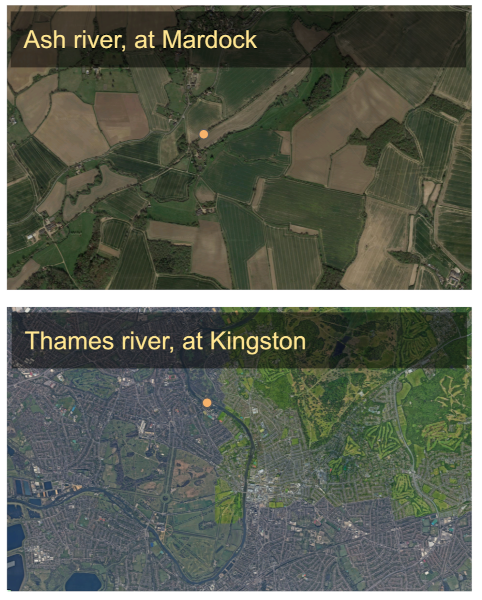
\includegraphics[width=0.6\textwidth,height=\textheight]{man/figures/riverCatchments.png}
\caption{\textbf{Fig 1:} Ariel images of the Ash, and Thames rivers}
\end{figure}

\textbf{Quick summary on inputs}\\
i. Evenly spaced series data (eg. can be time or space series)\\
ii. Label of the measurements taken. (eg. can be shape or signal
intensity)\\
iii. Labels for the objects to be compared (eg. cytoplasm and nuclear
compartments)\\
iv. Higher level groupings for comparing objects (eg. compare objects
per cell/organism/treatment/community)

\textbf{Quick notes on outputs}\\
i. Plots of calculated correlations clustered by strength at lag zero\\
ii. Plots of calculated asymmetries between past and future lags,
clustered by strength of asymmetry\\
iii. Plots representing both the strength of correlation at lag zero,
and the direction of correlation\\
iv. Calculated summary statistics of CCFs that can be used in downstream
analysis (e.g to improve the performance of classification tasks)

\hypertarget{detailed-examples}{%
\subsection{\texorpdfstring{\textbf{Detailed
examples}}{Detailed examples}}\label{detailed-examples}}

\textbf{description of default data} lifeTimes makes it easy to detect
``coupling'' between different components of biological systems from the
scale of cells, to organisms, to ecosystems. Along these lines,
lifeTimes comes with examples of:\\
i.landscape scale datasets, ii.subcellular scale datasets.

\hypertarget{dataset-1-rainfall-and-river-flow}{%
\subsection{\texorpdfstring{\textbf{Dataset 1: Rainfall and river
flow}}{Dataset 1: Rainfall and river flow}}\label{dataset-1-rainfall-and-river-flow}}

\protect\hyperlink{}{Back to top}

\textbf{Landscape scale data} lifeTimes can be used to find coupling
between processes at the landscape or ecosystem scale. For this example,
I have used data from the United Kingdom, National River Flow Archive
(\url{https://nrfa.ceh.ac.uk/web-download-service}). We will look at two
types of data, i) Gauged Daily Flows (GDF) which measure how much water
is in a river, and ii) Catchment Daily Rainfall (CDR) which measure the
amount of rain on the landscape around the river. River flows are in
cubic meters per second, and rainfall is in mm across the catchment in
the given reference period
(\url{https://nrfa.ceh.ac.uk/data-formats-types}).\\

For this example I have downloaded data from the Thames river, at
Kingston (\url{https://nrfa.ceh.ac.uk/data/station/info/39001}), and the
Ash river, at Mardock
\url{https://nrfa.ceh.ac.uk/data/station/info/38002}. I have also subset
the data between the years 1983 and 2017. This is a period where both
stations were operating, and recording measurements.\\

After some data wrangling, these two datsets produce a csv which I read
into a dataframe. The first five observations look like this:

\begin{Shaded}
\begin{Highlighting}[]
\NormalTok{rain\_flow }\OtherTok{\textless{}{-}} \FunctionTok{read.csv}\NormalTok{(}\AttributeTok{file =}\StringTok{"data{-}raw/rain\_flow\_Thames\_Ash.csv"}\NormalTok{)}
\FunctionTok{head}\NormalTok{(rain\_flow)}
\end{Highlighting}
\end{Shaded}

\begin{verbatim}
##         date dateAsInteger catchmentRegion flow_m3s rainfall_cm year month day
## 1 1983-06-01          4899  Ash at Mardock    4.720           3 1983     6   1
## 2 1983-06-02          4900  Ash at Mardock    0.756          12 1983     6   2
## 3 1983-06-03          4901  Ash at Mardock    0.543           8 1983     6   3
## 4 1983-06-04          4902  Ash at Mardock    0.450           0 1983     6   4
## 5 1983-06-05          4903  Ash at Mardock    0.392           0 1983     6   5
## 6 1983-06-06          4904  Ash at Mardock    0.363           0 1983     6   6
##   yearNumber dayNumber Reset_SeasonYearDay dayOfYear season dayOfseason
## 1          1       365                   0         0 summer           0
## 2          1       366                   1         1 summer           1
## 3          1       367                   2         2 summer           2
## 4          1       368                   3         3 summer           3
## 5          1       369                   4         4 summer           4
## 6          1       370                   5         5 summer           5
##                catchRep              uniqueID key_num
## 1 year_1_Ash at Mardock 1Ash at Mardocksummer  key_83
## 2 year_1_Ash at Mardock 1Ash at Mardocksummer  key_83
## 3 year_1_Ash at Mardock 1Ash at Mardocksummer  key_83
## 4 year_1_Ash at Mardock 1Ash at Mardocksummer  key_83
## 5 year_1_Ash at Mardock 1Ash at Mardocksummer  key_83
## 6 year_1_Ash at Mardock 1Ash at Mardocksummer  key_83
\end{verbatim}

Plotting the river flow and rainfall measures over a 1000 day interval
looks like this:
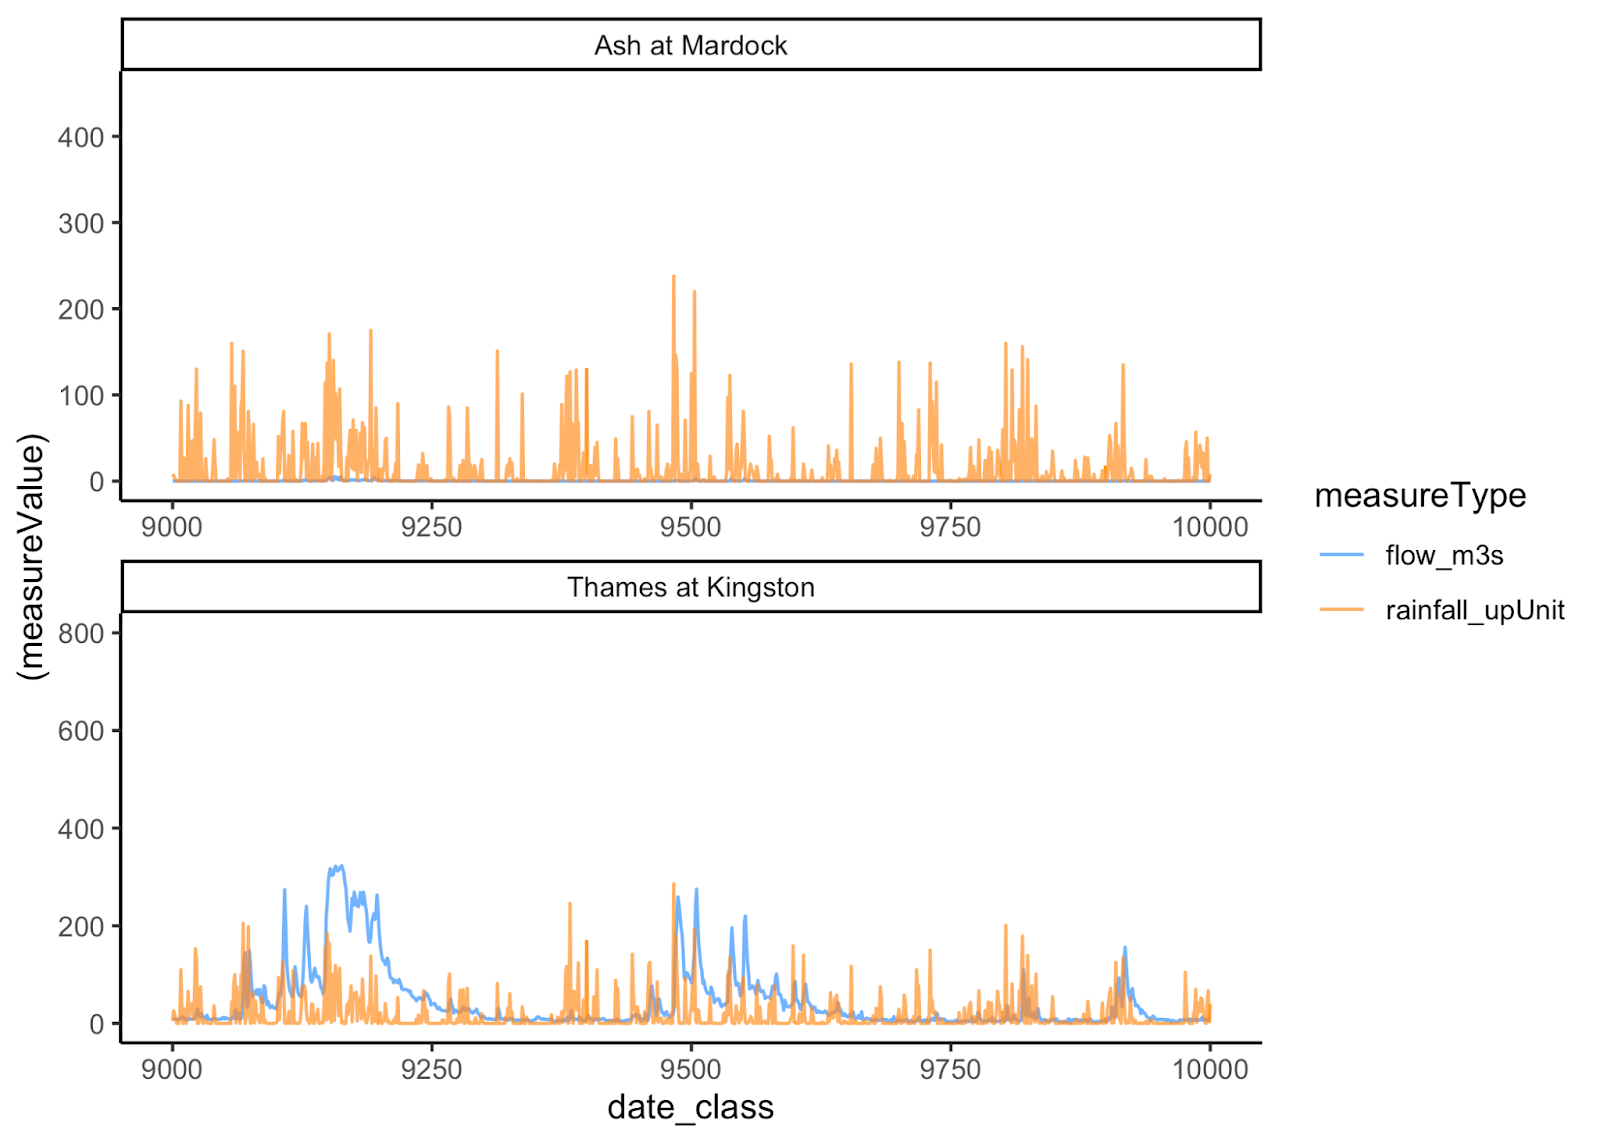
\includegraphics[width=1\textwidth,height=\textheight]{man/figures/raw_flow_rain.png}

The main funtion for user input in lifeTimes is \texttt{lts\_in()}. To
test that lifeTimes is working you can run this function without any
arguments. This will run the program on a default set of data.However,
it is more interesting to run lifeTimes on your own data. Below, I have
included a worked example of how to use run lifeTimes on a dataset. For
this example, I am still usingthe rain\_flow dataset, except that the
steps to run this data in \texttt{lts\_in()} are now clearly shown.

\textbf{Example 1}

\begin{Shaded}
\begin{Highlighting}[]
\FunctionTok{library}\NormalTok{(lifeTimes) }\CommentTok{\#load lifeTimes namespace}

\CommentTok{\#use the lts\_pairsMaker hrlper function }
\CommentTok{\#to prepare variables to be compared in a list of lists format }
\NormalTok{lts\_pairedVars }\OtherTok{\textless{}{-}} \FunctionTok{lts\_pairsMaker}\NormalTok{(}\FunctionTok{c}\NormalTok{(}\StringTok{"rainfall\_cm"}\NormalTok{,}\StringTok{"flow\_m3s"}\NormalTok{))}
\NormalTok{lts\_pairedVars}
\end{Highlighting}
\end{Shaded}

\begin{verbatim}
## $rainfall_cm
## $rainfall_cm[[1]]
## [1] "rainfall_cm"
## 
## $rainfall_cm[[2]]
## [1] "flow_m3s"
\end{verbatim}

\hypertarget{two-categorical-variable-with-single-pair-of-measured-variables}{%
\subsubsection{\texorpdfstring{\textbf{Two categorical variable with
single pair of measured
variables}}{Two categorical variable with single pair of measured variables}}\label{two-categorical-variable-with-single-pair-of-measured-variables}}

\protect\hyperlink{}{Back to top}

\begin{Shaded}
\begin{Highlighting}[]
\CommentTok{\#arguments for lts\_in() with default inputs (the "river catchments "rain\_flow" dataset) shown}
\FunctionTok{lts\_in}\NormalTok{(}\AttributeTok{.in\_tsData =}\NormalTok{ rain\_flow  , }\CommentTok{\#1. the dataset}
         \AttributeTok{.in\_time =} \FunctionTok{c}\NormalTok{(}\StringTok{"dayOfseason"}\NormalTok{), }\CommentTok{\#2. the time column}
       \AttributeTok{.in\_compare\_categorical =}  \FunctionTok{c}\NormalTok{(}\StringTok{"season"}\NormalTok{, }\StringTok{"catchmentRegion"}\NormalTok{), }\CommentTok{\#3. A vector, with the names of categorical columns}
       \AttributeTok{.in\_plot\_measured\_variables =} \ConstantTok{FALSE}\NormalTok{ , }\CommentTok{\#4. Whether to CCFs for multiple pairs of variables }
       \AttributeTok{.in\_pairedComparisons =}  \FunctionTok{list}\NormalTok{(}\AttributeTok{pair\_1 =} \FunctionTok{list}\NormalTok{(}\AttributeTok{y =} \StringTok{"rainfall\_cm"}\NormalTok{, }
        \AttributeTok{x =} \StringTok{"flow\_m3s"}\NormalTok{)), }\CommentTok{\#5. A list of lisys, holding the pairs of variables to be compared}
       \AttributeTok{.in\_uniqueID\_colname =} \StringTok{"key\_num"}\NormalTok{, }\CommentTok{\#6. The column with unique ID name for your observations}
       \AttributeTok{.in\_metaData =} \ConstantTok{NULL}\NormalTok{) }\CommentTok{\#7. Column names of any attributes you would like to append to data}
\end{Highlighting}
\end{Shaded}

I will now give a walkthrough that explains the arguments above, and how
to run lifeTimes, on your own data! To make any data suitable for
lifeTimes, we need the raw data, and four types labels which identify
the ``time'',``unique ID'', ``categorical variable'' and ``measured
variable'' columns. There is also an option to identify metadata:

\textbf{The Arguments}

\textbf{1:\texttt{.in\_tsData\ =} A series dataframe:} Time series
measurements. These should have:\\
i. at least two variables,\\
ii. evenly spaced intervals,\\
iii. Complete sets of observations (e.g NAs, can be imputed).\\
iv. Time series of equal length.\\
v. At least two categorical variables (e.g Treatment vs Control)

TODO: lifeTimes will be compatible with orical variable, and missing
observations. A helper function to impute NAs will also be included.

\textbf{2: \texttt{.in\_time\ =} A unit of time:} So we need to find the
column in the dataset that indicates this. In this data we have years,
months and days, but the unit of time I am interested in is at the
resolution of days. The column in the datset with days is called
\texttt{"dayOfseason"}. On the first day of each season (summer, autumn,
winter, spring) this value starts at one and increments up until the end
of the season.

\textbf{3: \texttt{.in\_compare\_categorical\ =} Categorical Variables:}
This is where you tell lifeTimes which colums hold the labels for
categorical variables. For example these might be experimental
treatments or conditions. Currently you can have 1 or 2 categorical
variables. For the rainflow dataset there are 2 columns with categorical
variables, and they are ``season'' (e.g a label that is `summer',
`autumn', `winter' or `spring') and ``catchmentRegion'' e.g ``Ash at
Mardock'' or ``Thames at Kingston''. LifeTimes will cluster your
categorical data based on correlations between measured variables.

\textbf{4: \texttt{.in\_plot\_measured\_variables\ =} Whether to plot
multiple variables?} This parameter takes a logical argument and can be
either ``TRUE'' or ``FALSE''. The choice depends on whether you are
analysing two categorical variables, in which case set it to ``FALSE''.
If you are studying one categorical variable but would like to calculate
and plot the cross correlations of multiple mesured variables, set this
to ``TRUE''. A detailed explanation is below.\\

Currently in lifeTimes, categorical and measured variables can be used
in two ways:\\

\begin{enumerate}
\def\labelenumi{\roman{enumi}.}
\tightlist
\item
  You can analyse 2 categorical variables and one pair of measured
  variables. This is shown with the ``rain\_flow'' dataset. The two
  categorical variables are ``catchment'' and ``season'', and the pair
  of measured variables are ``rainfall\_cm'' and ``flow\_m3s''.\\
\item
  alternatively, if you are using one categorical variable, but more
  than one pair of measured variablesyou can set this to
  \texttt{.in\_plot\_measured\_variables\ =\ TRUE}
\end{enumerate}

\textbf{5: \texttt{.in\_pairedComparisons\ =} Pairs of variables to
compare to one another at different lags:} Under the hood, these are
passed to the lifeTimes internal functions in the format of a list of
lists. There is one master list, holding lists of paired variables to
compare. In practice, there is a helper fuction
\texttt{lts\_pairsMaker()}, that takes a vector with a list of column
names, and returns all possible non redundant pairs of variables in this
list. So you can give a list of variables you would like to compare to
the \texttt{lts\_pairsMaker} function, and assign the output to an
object. Then just pass this object as an argument to the
\texttt{.in\_pairedComparisons\ =} parameter (See example 1 above). In
addition to iterating all possible combinations of pairings between
variables, lts\_pairsMaker can be passed a table of pre-specified
pairings, and return these in list of list format (this is demonstrated
in the examples below).

\textbf{6:\texttt{.in\_uniqueID\_colname\ =} A unique identified for
each thing we are measuring:} We need to give lifeTimes the column namr
which holds the unique identifier for each observation. If there isn,t
one, we can create a column in the data frame with unique identifier for
each observation.\\

In this dataset the column is called ``key\_num''. In general, an unit
of observation is some unit of interest, measured over time. In this
dataset, it's a river measuring station, in a given season, in a given
year. For example, ``Ash river in summer in 1995'', or ``Thames river in
winter of 2001''. So in this dataset I have grouped the data by,
River,Season and Year, and given a unique ID to each observation and
labelled the column \texttt{"key\_num"}.\\

TODO: Future updates to lifetimes will include a helper function that
inputs a set of columns defining a unique observation, and outputs
creates a new column of uniqueIDs.

\textbf{7: \texttt{.in\_metaData\ =} Column names of metadata:} This
parameter takes column names of any attributes you would like to append
to data

\hypertarget{dataset-2-cell-and-nucleus}{%
\subsection{\texorpdfstring{\textbf{Dataset 2: Cell and
nucleus}}{Dataset 2: Cell and nucleus}}\label{dataset-2-cell-and-nucleus}}

\protect\hyperlink{}{Back to top}

\textbf{Subcellular scale data} We have seen that lifeTimes can be used
to detect the coupling between lanscape scale processes such as rainfall
and riverflow, and to highlight how this coupling varies between seasons
and geographical regions. In this next example, I am using lifeTimes to
look at coupling between the overall geometry of a living cell, and the
nucleus compartment within that cell. For this example I have used data
from melanoma cells imaged in a 3D collagen matrix, treated with
different drugs that affect cell function. The data here are just 30
cells (5 cells for each drug treatment), sampled for demonstration
purposes, from a larger dataset.\\

First I read in the `sampleCells.csv' data, that is included in the
lifeTimes package.

\begin{Shaded}
\begin{Highlighting}[]
\DocumentationTok{\#\#\#start example}
\NormalTok{lts\_cells }\OtherTok{\textless{}{-}} \FunctionTok{read.csv}\NormalTok{(}\AttributeTok{file =} \StringTok{"data{-}raw/sampleCells.csv"}\NormalTok{)}
\end{Highlighting}
\end{Shaded}

Next, I look at the column names to see the categorical variables, and
measured variables in the dataset

\begin{Shaded}
\begin{Highlighting}[]
\CommentTok{\#look at colum names}
\FunctionTok{colnames}\NormalTok{(lts\_cells)}
\end{Highlighting}
\end{Shaded}

\begin{verbatim}
##  [1] "Volume_cell"                "EquivDiameter"             
##  [3] "SurfaceArea_cell"           "MeanIntensity"             
##  [5] "MinIntensity"               "MaxIntensity"              
##  [7] "MajorAxis_cell"             "MinorAxis_cell"            
##  [9] "secondMajor_cell"           "Eccentricity_cell"         
## [11] "secondEccentricity_cell"    "Sphericity_cell"           
## [13] "Vol2surf_cell"              "runNumber"                 
## [15] "timeTrack"                  "yDim"                      
## [17] "xDim"                       "zDim"                      
## [19] "xCoord_cell"                "yCoord_cell"               
## [21] "zCoord_cell"                "Orbit"                     
## [23] "AngleBetween"               "serialNumber"              
## [25] "nProtrusions_cell"          "CoverslipPresent"          
## [27] "CoverslipDistance"          "OnCoverslip"               
## [29] "fieldNumber"                "Treatment"                 
## [31] "Row"                        "Column"                    
## [33] "Polarity_cell"              "Spreading_cell"            
## [35] "Protrusivity_cell"          "cellNumber"                
## [37] "NucleusVolumeFraction"      "Volume_nucleus"            
## [39] "SurfaceArea_nucleus"        "MajorAxis_nucleus"         
## [41] "MinorAxis_nucleus"          "secondMajor_nucleus"       
## [43] "Eccentricity_nucleus"       "secondEccentricity_nucleus"
## [45] "Sphericity_nucleus"         "Vol2surf_nucleus"          
## [47] "xCoord_nucleus"             "yCoord_nucleus"            
## [49] "zCoord_nucleus"             "nProtrusions_nucleus"      
## [51] "Polarity_nucleus"           "Spreading_nucleus"         
## [53] "Protrusivity_nucleus"       "Plate"                     
## [55] "cluster"
\end{verbatim}

Here, I can see that \texttt{"runNumber"}, will be the column with the
time information, and \texttt{"cellNumber"} will be the unique ID for
each observation. \texttt{"Treatment"} is a categorical variable.

For this dataset, I am only interested in one categorical variable,
called ``Treatment''. This variable describes the drug that each cell
has been exposed to. This is in contrast to the ``rain\_flow'' dataset
(example 1 above) where there were two categorical variables of inerest
(``season'' and ``catchmentRegion'').\\

Also, I can see that there are many measured variables for both the cell
and nucleus that I could compare (eg. ``Polarity\_cell'',
``Eccentricity\_nucleus'', ``Volume\_cell'' etc.) . This is in contrast
to the ``rain\_flow'' dataset where there were only two measured
variables.\\

\textbf{User defined paired comparisons} For this dataset, instead of
using \texttt{lts\_pairsMaker} to permute all the possible comparisons
between measured variables, I will specifically define the variables to
compare. In the cell dataset, we can use some domain specific knowledge
to recognise that comparing the coupling of geometry between the cell
and nucleus under different drug treatments is meaningful and
interesting. To make this comparisons, I have just listed some of the
features I would like to directly compare, and then joined this into a
matrix that I named \texttt{my\_pairs} by using \texttt{rbind()}:

\begin{Shaded}
\begin{Highlighting}[]
\CommentTok{\#choose three pairs of column names}
\NormalTok{pair1 }\OtherTok{\textless{}{-}} \FunctionTok{c}\NormalTok{(}\StringTok{"Polarity\_cell"}\NormalTok{,}\StringTok{"Polarity\_nucleus"}\NormalTok{)}
\NormalTok{pair2 }\OtherTok{\textless{}{-}} \FunctionTok{c}\NormalTok{(}\StringTok{"Eccentricity\_cell"}\NormalTok{, }\StringTok{"Eccentricity\_nucleus"}\NormalTok{)}
\NormalTok{pair3 }\OtherTok{\textless{}{-}} \FunctionTok{c}\NormalTok{(}\StringTok{"Volume\_cell"}\NormalTok{, }\StringTok{"Volume\_nucleus"}\NormalTok{)}

\CommentTok{\# use rbind to make these pairs into a matrix}
\NormalTok{my\_pairs }\OtherTok{\textless{}{-}} \FunctionTok{rbind}\NormalTok{(pair1,pair2,pair3)}
\end{Highlighting}
\end{Shaded}

I passed \texttt{my\_pairs} to \texttt{lts\_pairsMaker} with
\texttt{defined\ =\ TRUE}, to create a list of specific paired
comparisons that I would like to make. This contrasts with the less
default use of \texttt{lts\_pairsMaker}, where a list of column names is
entered, and all possible non-redundant combinations of these are
returned.

\begin{Shaded}
\begin{Highlighting}[]
\CommentTok{\#make these into list of pairs using helper function with "defined = TRUE"}
\NormalTok{lts\_pairs }\OtherTok{\textless{}{-}} \FunctionTok{lts\_pairsMaker}\NormalTok{(my\_pairs, }\AttributeTok{defined =} \ConstantTok{TRUE}\NormalTok{)}
\end{Highlighting}
\end{Shaded}

\hypertarget{single-categorical-variable-with-multiple-measured-variables}{%
\subsubsection{\texorpdfstring{\textbf{Single categorical variable with
multiple measured
variables}}{Single categorical variable with multiple measured variables}}\label{single-categorical-variable-with-multiple-measured-variables}}

\protect\hyperlink{}{Back to top}

The data, relevant column names and list of pairs can all be entered
into \texttt{lts\_in()}. The important and interesting difference
between this example and the ``rain\_flow'' example, is that we are now
using a \textbf{single categorical variable}, ``Treatment''. In this
situation you must set \texttt{.in\_plot\_measured\_variables\ =\ TRUE}.
This means lifeTimes will cluster and plot the different measured
variables.\\

TODO: Improve UI by either removing
\texttt{.in\_plot\_measured\_variables\ =\ TRUE} argument, and making it
automatic when only one categorical is entered, OR make it possible to
enter only one categorical, while
\texttt{.in\_plot\_measured\_variables\ =\ FALSE}.

\begin{Shaded}
\begin{Highlighting}[]
\CommentTok{\# enter arguments into lts\_in}
\CommentTok{\# here there is one categorical variable and multiple measured variables}
\NormalTok{lts\_oneCat }\OtherTok{\textless{}{-}} \FunctionTok{lts\_in}\NormalTok{(}\AttributeTok{.in\_tsData =}\NormalTok{ lts\_cells,}
                     \AttributeTok{.in\_compare\_categorical =} \StringTok{"Treatment"}\NormalTok{,}
                     \AttributeTok{.in\_time =} \StringTok{"runNumber"}\NormalTok{,}
                     \AttributeTok{.in\_plot\_measured\_variables =} \ConstantTok{TRUE}\NormalTok{,}
                     \AttributeTok{.in\_pairedComparisons =}\NormalTok{ lts\_pairs,}
                     \AttributeTok{.in\_uniqueID\_colname =} \StringTok{"cellNumber"}\NormalTok{,}
                     \AttributeTok{.in\_metaData =} \ConstantTok{NULL}\NormalTok{ )}
\end{Highlighting}
\end{Shaded}

After running \texttt{lts\_in()}, the output can be plotted with the
three lifeTimes plotting functions. Examples are below:

\begin{Shaded}
\begin{Highlighting}[]
\CommentTok{\#View results}
\FunctionTok{lts\_plot\_ccfs}\NormalTok{(lts\_oneCat)}
\end{Highlighting}
\end{Shaded}

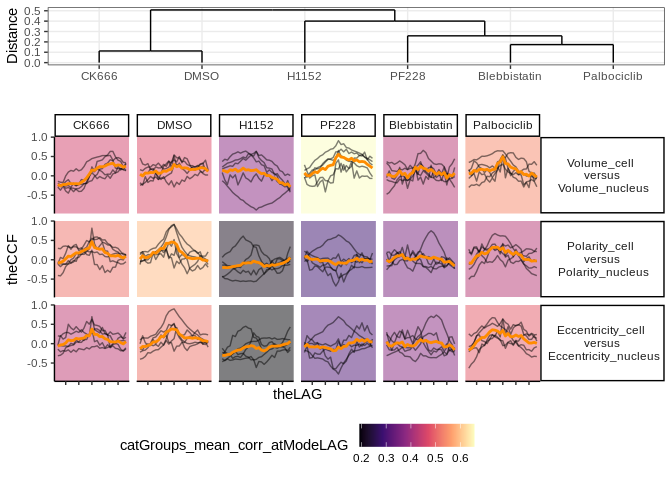
\includegraphics{htmlREADME_files/figure-latex/unnamed-chunk-12-1.pdf}

\begin{Shaded}
\begin{Highlighting}[]
\FunctionTok{lts\_plot\_ClustSum}\NormalTok{(lts\_oneCat)}
\end{Highlighting}
\end{Shaded}

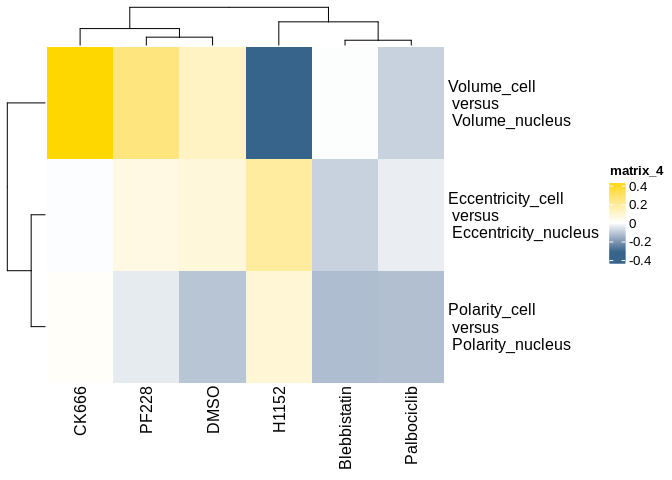
\includegraphics{htmlREADME_files/figure-latex/unnamed-chunk-12-2.pdf}

This example of \texttt{lts\_plot\_coupled()} shows two plots of the
same data, and how the colouring and faceting variables can be switched
with the \texttt{.lts\_colour\_by\ =} and `.lts\_facet\_by =```
parameters.

\begin{Shaded}
\begin{Highlighting}[]
\FunctionTok{lts\_plot\_coupled}\NormalTok{(lts\_oneCat, }
                 \AttributeTok{.lts\_colour\_by =} \StringTok{"cat1"}\NormalTok{, }
                 \AttributeTok{.lts\_facet\_by =} \StringTok{"cat2"}\NormalTok{)}
\end{Highlighting}
\end{Shaded}

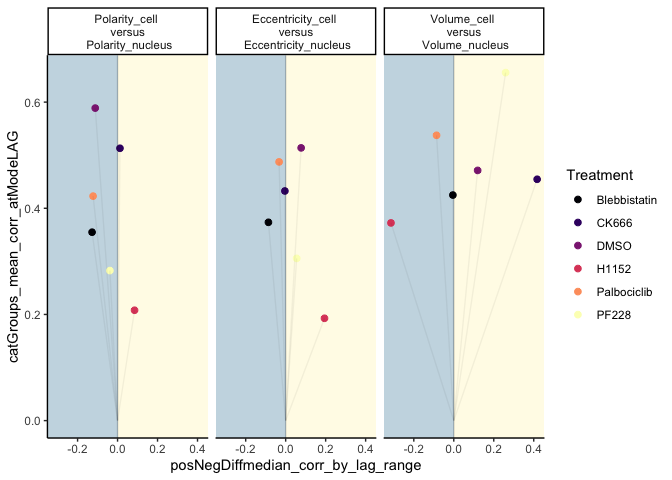
\includegraphics{htmlREADME_files/figure-latex/unnamed-chunk-13-1.pdf}

\begin{Shaded}
\begin{Highlighting}[]
\FunctionTok{lts\_plot\_coupled}\NormalTok{(lts\_oneCat, }
                 \AttributeTok{.lts\_colour\_by =} \StringTok{"cat2"}\NormalTok{, }
                 \AttributeTok{.lts\_facet\_by =} \StringTok{"cat1"}\NormalTok{)}
\end{Highlighting}
\end{Shaded}

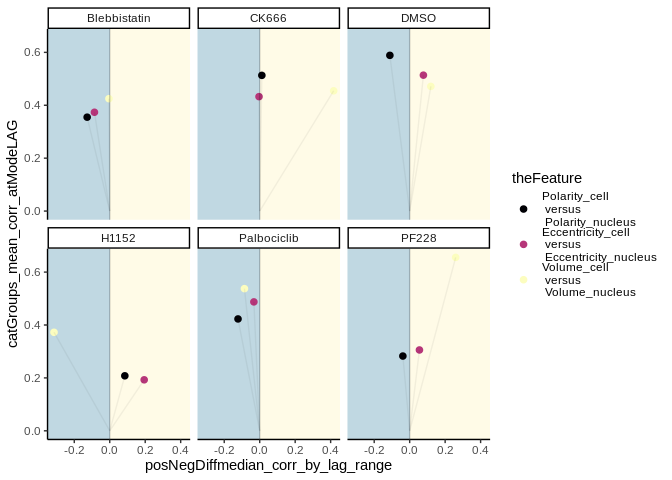
\includegraphics{htmlREADME_files/figure-latex/unnamed-chunk-13-2.pdf}

\hypertarget{downstream-analysis-rainfall-and-river-flow}{%
\subsection{\texorpdfstring{\textbf{Downstream analysis: Rainfall and
river
flow}}{Downstream analysis: Rainfall and river flow}}\label{downstream-analysis-rainfall-and-river-flow}}

\protect\hyperlink{}{Back to top}

Cross correlations, or lagged correlations between features have many
uses. Two of these are:\\
i. generating hypotheses about cause and effect between parts of a
system\\
ii. improving the results of classification tasks indynamic datasets\\

The code below shows how you can access summary statistics about each
ovbservation, for use in downstream tasks.

\begin{Shaded}
\begin{Highlighting}[]
\CommentTok{\#load lideTimes}
\FunctionTok{library}\NormalTok{(lifeTimes)}

\CommentTok{\#run lifeTimes}
\NormalTok{lts\_demo }\OtherTok{\textless{}{-}} \FunctionTok{lts\_in}\NormalTok{()}
\end{Highlighting}
\end{Shaded}

\hypertarget{output-summary-statistics}{%
\subsubsection{\texorpdfstring{\textbf{Output summary
statistics}}{Output summary statistics}}\label{output-summary-statistics}}

\protect\hyperlink{}{Back to top}

lifeTimes outputs a range of ccf summary statistics. These are stored in
a list called ``lts\_ccf\_summaries''.

\begin{Shaded}
\begin{Highlighting}[]
\CommentTok{\#Here is an example of accessing one set of summary statistics}
\CommentTok{\#and assigning it to an object}
\NormalTok{lts\_summary\_output }\OtherTok{\textless{}{-}}\NormalTok{ lts\_demo}\SpecialCharTok{$}\NormalTok{lts\_ccf\_summaries}\SpecialCharTok{$}\NormalTok{lts\_singleton\_summ\_metadata}
\end{Highlighting}
\end{Shaded}

\textbf{summary cleaning functions} lifeTimes has a built in function
\texttt{lts\_summs\_clean()}, to clean summary statistics for downstream
analysis. This function just takes the output of the \texttt{lts\_in()}
function.

\begin{Shaded}
\begin{Highlighting}[]
\CommentTok{\#Just enter the output from lts\_in(), into the lts\_summs\_clean() function}
\NormalTok{lts\_clean\_demo }\OtherTok{\textless{}{-}} \FunctionTok{lts\_summs\_clean}\NormalTok{(lts\_demo)}
\end{Highlighting}
\end{Shaded}

This attaches a list called \texttt{"lts\_clean\_summs"} to the
\texttt{lts\_in()} output, which contains:

\begin{enumerate}
\def\labelenumi{\roman{enumi}.}
\item
  summary statistics of original time series input, called
  \texttt{lts\_clean\_summ\_original}
\item
  summary statistics of ccf calculations, called
  \texttt{lts\_clean\_summ\_ccf}
\item
  a join of both (i) and (ii), to give combined summary statistics,
  \texttt{lts\_clean\_summ\_join}\\

  This new list can be passed to \texttt{lts\_prcomp()}, to generate
  principle components.
\end{enumerate}

\begin{Shaded}
\begin{Highlighting}[]
\CommentTok{\#Use lapply to iterate over "lts\_clean\_summs", to generate principle components}
\NormalTok{lts\_pc\_list }\OtherTok{\textless{}{-}} \FunctionTok{lapply}\NormalTok{(lts\_clean\_demo}\SpecialCharTok{$}\NormalTok{lts\_clean\_summs, lts\_prcomp) }\CommentTok{\#run pc analyis on each}
\end{Highlighting}
\end{Shaded}

\hypertarget{visualising-principal-component-space}{%
\subsubsection{\texorpdfstring{\textbf{Visualising principal component
space}}{Visualising principal component space}}\label{visualising-principal-component-space}}

\protect\hyperlink{}{Back to top}

Principle component space can be plotted for each of the three summary
statistics. First we install the needed packages. Then we assign labels,
and use lapply on our already computed principle components. This
generates a list of plots.

\begin{Shaded}
\begin{Highlighting}[]
\CommentTok{\#install ggfortify if needed}
\ControlFlowTok{if}\NormalTok{(}\SpecialCharTok{!}\FunctionTok{require}\NormalTok{(}\StringTok{"ggfortify"}\NormalTok{)) }\FunctionTok{install.packages}\NormalTok{(}\StringTok{"ggfortify"}\NormalTok{)}
\end{Highlighting}
\end{Shaded}

\begin{verbatim}
## Loading required package: ggfortify
\end{verbatim}

\begin{verbatim}
## Loading required package: ggplot2
\end{verbatim}

\begin{Shaded}
\begin{Highlighting}[]
\FunctionTok{library}\NormalTok{(ggfortify)}

\CommentTok{\#make labels}
\NormalTok{lts\_pca\_labels }\OtherTok{\textless{}{-}}\NormalTok{ lts\_pc\_list}\SpecialCharTok{$}\NormalTok{lts\_clean\_summ\_original}\SpecialCharTok{$}\NormalTok{lts\_labels\_pc}

\CommentTok{\#make 3 versions of PCA space}
\NormalTok{p }\OtherTok{\textless{}{-}} \FunctionTok{lapply}\NormalTok{(lts\_pc\_list, }\ControlFlowTok{function}\NormalTok{(x) }\FunctionTok{autoplot}\NormalTok{(x}\SpecialCharTok{$}\NormalTok{lts\_pc\_values, }
                                              \AttributeTok{data =}\NormalTok{lts\_pca\_labels,     }
                                              \AttributeTok{colour =} \StringTok{"catchmentRegion"}\NormalTok{)}\SpecialCharTok{+}
  \FunctionTok{scale\_color\_manual}\NormalTok{(}\AttributeTok{values =} \FunctionTok{c}\NormalTok{(}\StringTok{"dodgerblue"}\NormalTok{,}\StringTok{"darkorange"}\NormalTok{))}\SpecialCharTok{+}  \FunctionTok{theme\_classic}\NormalTok{())}
\end{Highlighting}
\end{Shaded}

Principle component space can be plotted for each of the three summary
statistics:\\
i. original data summaries

\begin{enumerate}
\def\labelenumi{\roman{enumi}.}
\setcounter{enumi}{1}
\item
  calculated ccfs summaries
\item
  combined data summaries
\end{enumerate}

\begin{Shaded}
\begin{Highlighting}[]
\CommentTok{\#plot PCA space}
\ControlFlowTok{if}\NormalTok{(}\SpecialCharTok{!}\FunctionTok{require}\NormalTok{(}\StringTok{"gridExtra"}\NormalTok{)) }\FunctionTok{install.packages}\NormalTok{(}\StringTok{"gridExtra"}\NormalTok{)}
\end{Highlighting}
\end{Shaded}

\begin{verbatim}
## Loading required package: gridExtra
\end{verbatim}

\begin{Shaded}
\begin{Highlighting}[]
\FunctionTok{library}\NormalTok{(gridExtra)}
\FunctionTok{do.call}\NormalTok{(}\StringTok{"grid.arrange"}\NormalTok{, p)}
\end{Highlighting}
\end{Shaded}

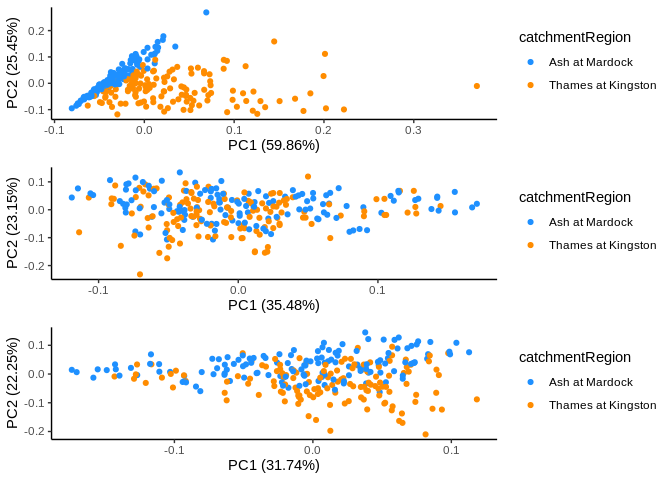
\includegraphics{htmlREADME_files/figure-latex/unnamed-chunk-19-1.pdf}

In comparison to the original data, the combined dataset give improved
performance in classification tasks. Importantly, this improvement comes
from the same original data without the addition of any new variables or
measures. Instead, the improvement comes from the CCFs which give a
better account of the relationship or coupling between measured
variables and how these change between conditions.

\hypertarget{using-plsr-to-predict-catchment-location}{%
\subsubsection{\texorpdfstring{\textbf{Using PLSR to predict catchment
location}}{Using PLSR to predict catchment location}}\label{using-plsr-to-predict-catchment-location}}

\protect\hyperlink{}{Back to top}

We can look at performance in classification tasks using PLSR to predict
\texttt{catchmentRegion}, as a dummy variable. First we install and load
the ``pls'' package.

\begin{Shaded}
\begin{Highlighting}[]
\ControlFlowTok{if}\NormalTok{(}\SpecialCharTok{!}\FunctionTok{require}\NormalTok{(}\StringTok{"pls"}\NormalTok{)) }\FunctionTok{install.packages}\NormalTok{(}\StringTok{"pls"}\NormalTok{)}
\end{Highlighting}
\end{Shaded}

\begin{verbatim}
## Loading required package: pls
\end{verbatim}

\begin{verbatim}
## 
## Attaching package: 'pls'
\end{verbatim}

\begin{verbatim}
## The following object is masked from 'package:stats':
## 
##     loadings
\end{verbatim}

\begin{Shaded}
\begin{Highlighting}[]
\FunctionTok{library}\NormalTok{(pls)}
\end{Highlighting}
\end{Shaded}

\textbf{Original data summary stats}

From summary statistics of original data, CV analysis suggests 4 comps
be used. This gives prediction accuracy of \texttt{66.74}.

\begin{Shaded}
\begin{Highlighting}[]
\CommentTok{\#get categorical variables and predictors}
\NormalTok{lts\_PLSR }\OtherTok{\textless{}{-}}\NormalTok{ lts\_pc\_list}\SpecialCharTok{$}\NormalTok{lts\_clean\_summ\_original}

\CommentTok{\#Get column names of predictors}
\NormalTok{lts\_predictors }\OtherTok{\textless{}{-}}\NormalTok{ lts\_PLSR}\SpecialCharTok{$}\NormalTok{lts\_values\_pc}
\NormalTok{lts\_response }\OtherTok{\textless{}{-}} \FunctionTok{as.numeric}\NormalTok{(lts\_PLSR}\SpecialCharTok{$}\NormalTok{lts\_labels\_pc}\SpecialCharTok{$}\NormalTok{catchmentRegion)}
\NormalTok{PLSR\_model }\OtherTok{\textless{}{-}} \FunctionTok{plsr}\NormalTok{(lts\_response }\SpecialCharTok{\textasciitilde{}}\NormalTok{ ., }\AttributeTok{data=}\NormalTok{lts\_predictors, }\AttributeTok{scale=}\ConstantTok{TRUE}\NormalTok{, }\AttributeTok{validation=}\StringTok{"CV"}\NormalTok{)}
\end{Highlighting}
\end{Shaded}

\textbf{Plot RMSEP and prediction accuracy with Original Data}

\begin{Shaded}
\begin{Highlighting}[]
\FunctionTok{plot}\NormalTok{(}\FunctionTok{RMSEP}\NormalTok{(PLSR\_model), }\AttributeTok{legendpos =} \StringTok{"topright"}\NormalTok{)}
\end{Highlighting}
\end{Shaded}

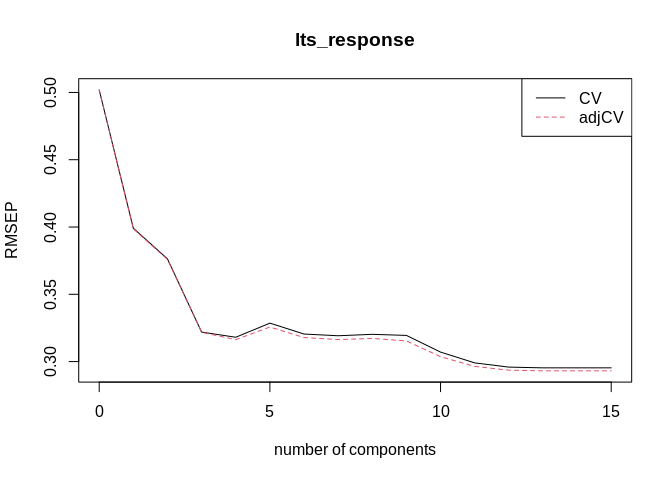
\includegraphics{htmlREADME_files/figure-latex/unnamed-chunk-22-1.pdf}

\begin{Shaded}
\begin{Highlighting}[]
\FunctionTok{plot}\NormalTok{(PLSR\_model)}\SpecialCharTok{+}\FunctionTok{abline}\NormalTok{(}\AttributeTok{h =}\FloatTok{1.5}\NormalTok{, }\AttributeTok{col =} \StringTok{"magenta"}\NormalTok{)}
\end{Highlighting}
\end{Shaded}

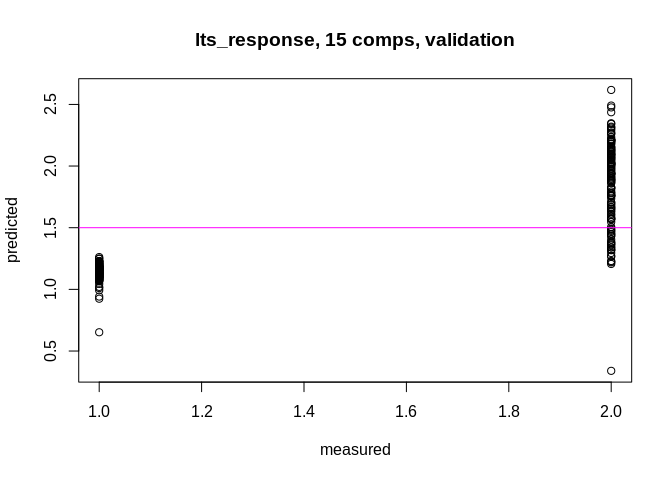
\includegraphics{htmlREADME_files/figure-latex/unnamed-chunk-22-2.pdf}

\begin{verbatim}
## numeric(0)
\end{verbatim}

\textbf{CCF + Original data summary stats}

From summary statistics of original and cross correlation data (CCF), CV
analysis suggests 8 comps be used. This gives prediction accuracy of
\texttt{75.35}.

\begin{Shaded}
\begin{Highlighting}[]
\CommentTok{\#get categorical variables and predictors}
\NormalTok{lts\_PLSR }\OtherTok{\textless{}{-}}\NormalTok{ lts\_pc\_list}\SpecialCharTok{$}\NormalTok{lts\_clean\_summ\_join}

\CommentTok{\#Get column names of predictors}
\NormalTok{lts\_predictors }\OtherTok{\textless{}{-}}\NormalTok{ lts\_PLSR}\SpecialCharTok{$}\NormalTok{lts\_values\_pc}
\NormalTok{lts\_response }\OtherTok{\textless{}{-}} \FunctionTok{as.numeric}\NormalTok{(lts\_PLSR}\SpecialCharTok{$}\NormalTok{lts\_labels\_pc}\SpecialCharTok{$}\NormalTok{catchmentRegion)}
\NormalTok{PLSR\_model }\OtherTok{\textless{}{-}} \FunctionTok{plsr}\NormalTok{(lts\_response }\SpecialCharTok{\textasciitilde{}}\NormalTok{ ., }\AttributeTok{data=}\NormalTok{lts\_predictors, }\AttributeTok{scale=}\ConstantTok{TRUE}\NormalTok{, }\AttributeTok{validation=}\StringTok{"CV"}\NormalTok{)}
\end{Highlighting}
\end{Shaded}

\textbf{Plot RMSEP and prediction accuracy with CCF Augmented Data}

\begin{Shaded}
\begin{Highlighting}[]
\FunctionTok{plot}\NormalTok{(}\FunctionTok{RMSEP}\NormalTok{(PLSR\_model), }\AttributeTok{legendpos =} \StringTok{"topright"}\NormalTok{)}
\end{Highlighting}
\end{Shaded}

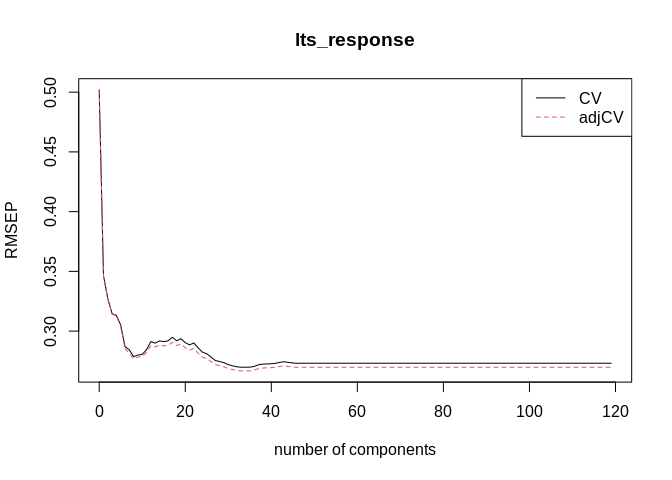
\includegraphics{htmlREADME_files/figure-latex/unnamed-chunk-24-1.pdf}

\begin{Shaded}
\begin{Highlighting}[]
\FunctionTok{plot}\NormalTok{(PLSR\_model)}\SpecialCharTok{+}\FunctionTok{abline}\NormalTok{(}\AttributeTok{h =}\FloatTok{1.5}\NormalTok{, }\AttributeTok{col =} \StringTok{"magenta"}\NormalTok{)}
\end{Highlighting}
\end{Shaded}

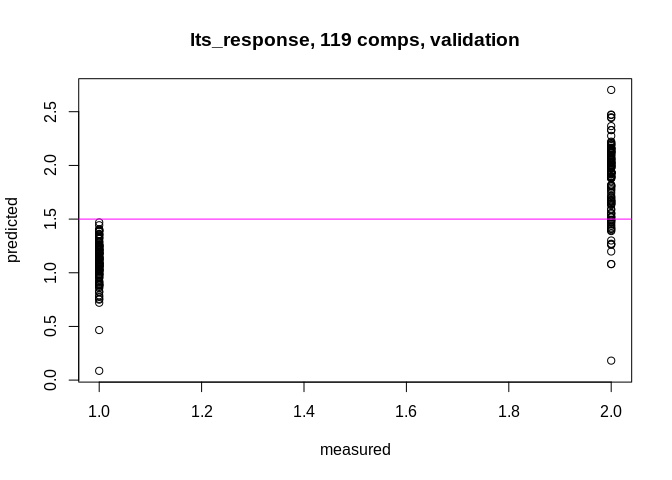
\includegraphics{htmlREADME_files/figure-latex/unnamed-chunk-24-2.pdf}

\begin{verbatim}
## numeric(0)
\end{verbatim}

In this simple example, using cross validated PLSR models, and selecting
the number of model components where RMSEP reaches the first turning
point, the improvement in prediction accuracy by incorporating CCF
summary statistics is \texttt{75.35\ -\ 66.74\ =\ 8.61}. This
improvement comes without adding any new measurements to the original
data. The improvement in prediction accuracy is likely to depend on
whether there are strong and characteristic difference in the
relationships between variables in your dataset, and whether these
differ between conditions.

\protect\hyperlink{}{Back to top}

© 2022 GitHub, Inc. Terms Privacy Security Status

\end{document}
